\chapter{pemahaman teori}
\section{apa itu fungsi file csv,sejarah csv dan contohnya}
\begin{enumerate}
	\item [a.]apa itu fungsi file csv
	        \par Comma Separated Value atau yang biasa dikenal dengan sebutan CSV ini adalah suatu format data yang dapat mempermudah penggunanya dalam melakukan penginputan data kedalam database yang dapat dilakukan dengan mudah dan sederhana. CSV sendiri  bisa digunakan  dalam standar file ASCII,dimana setiap file record yang ada dapat dipisahkan dengan tanda koma(,) atau tanda titik koma (;).
\item [b.]sejarah csv\\
\hspace*{1cm}	Comma-separated values adalah adalah format nilai yang dipisahkan oleh dataComma yang melakukan pra-tanggal pada komputer pribadi lebih dari satu decade. Pada tahun i972 IBM Fotran (level H extended)  compiler dibawah OS/360  pada saat itu telah mendukung adanya CSV.padasaat itu Fotran 77 mendefinisikan penulisan pada input/outputyang ditulis menggunakan tanda koma dan juga spasi untuk digunakan sebagai pembatas, sehingga string yang karakter yang tidak dikutip tidak dapat mengandung koma ataupun spasi.\\
\hspace*{1cm}  Nama "dipisahkan nilai koma" dan singkatan "CSV" digunakan pada tahun 1983. [8]  dilakukan  secara manual untuk komputer Osborne Executive, yang mem-bundle spreadsheet SuperCalc, mendokumentasikan konvensi kutipan CSV yang memungkinkan string mengandung koma yang disematkan, tetapi manual tersebut tidak menentukan konvensi untuk menanamkan tanda kutip dalam string yang dikutip. Daftar nilai yang dipisahkan koma lebih mudah untuk diketik (misalnya ke dalam kartu berlubang) daripada data yang selaras dengan kolom tetap, dan cenderung menghasilkan hasil yang salah jika suatu nilai dilubangi satu kolom dari lokasi yang dituju.\\
\hspace*{1cm} yang dipisahkan koma digunakan untuk pertukaran informasi basis data antara mesin dari dua arsitektur yang berbeda. Karakter teks-polos dari file CSV sebagian besar menghindari ketidakcocokan seperti urutan byte dan ukuran kata. File-file ini sebagian besar dapat dibaca oleh manusia, sehingga lebih mudah untuk mengatasinya tanpa adanya dokumentasi atau komunikasi yang sempurna. 
Inisiatif standardisasi utama — mentransformasikan "definisi fuzzy de facto" menjadi definisi yang lebih tepat dan de jure - adalah pada 2005, dengan RFC4180, mendefinisikan CSV sebagai Tipe Konten MIME. Kemudian, pada 2013, beberapa kekurangan RFC4180 ditangani oleh rekomendasi W3C. Pada tahun 2014 IETF menerbitkan RFC7111 yang menjelaskan aplikasi fragmen URI pada dokumen CSV. RFC7111 menentukan bagaimana rentang baris, kolom, dan sel dapat dipilih dari dokumen CSV menggunakan indeks posisi. Pada 2015 W3C, dalam upaya untuk meningkatkan CSV dengan semantik formal, mempublikasikan draft rekomendasi pertama untuk standar metadata CSV, yang dimulai sebagai rekomendasi pada bulan Desember tahun yang sama. 
\item[c.] contoh csv
\begin{lstlisting}
npm;nama;kelas
1.1184039;tari;2A
2. 1184022;echa;2B
3. 1184086;hanifah;2C
\end{lstlisting}
\end{enumerate}
\section{Aplikasi yang bisa menghasilkan file csv}
\begin{enumerate}
    \item [a.]  spreadsheet  (Microsoft excel,  libreoffice, google spreadshare dll.
	\item[b.] Editor teks (notepad, visual studio code, sublime dll.
\end{enumerate}
\section{Cara menulis dan membaca file csv pada excel atau spreadsheet}
\begin{enumerate}
    \item [a.]pertama-tamayang dilakukan adalah dengan membuka terlebih dahulu aplikasi Microsoft excel.
    \newpage
    \item[b.]kemudian setelah excel maka langkah selanjutnya adalah dengan mengisi data sesuai yang diinginkan.tampilannya bisa dilihat padagambar dibawah
     \begin{figure}[!htbp]
    \begin{center}
    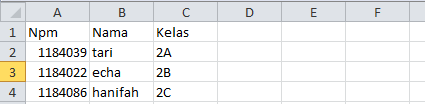
\includegraphics[width=9cm]{gambar/2.png}
    \end{center}   
    \end{figure}
    \item[c.]langkah selanjutnya adalah dengan memilih opsi file yang berada pada bagian pojokkiri atas, lalu pilih save and send.
     \begin{figure}[!htbp]
    \begin{center}
    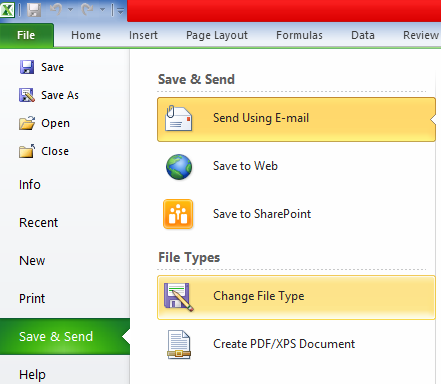
\includegraphics[width=9cm]{gambar/3.png}
    \end{center}   
    \end{figure}
    \newpage
    \item[d.]selanjutnya adalah pilih change file type, kemudian  pilih yang format CSV lalu klik Save as.
     \begin{figure}[!htbp]
    \begin{center}
    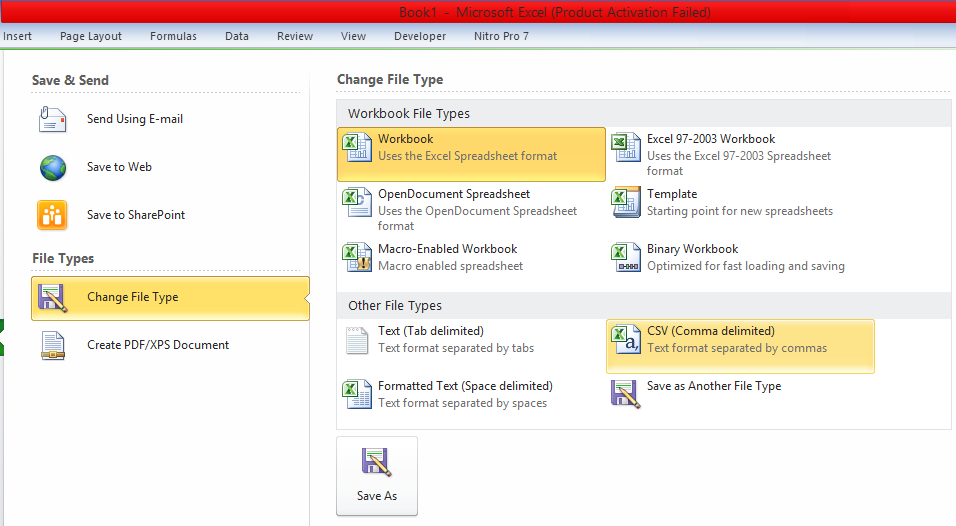
\includegraphics[width=9cm]{gambar/4.png}
    \end{center}   
    \end{figure}
     \item[e.]kemudian isi kolom file name dengan nama sesuai dengan data yang anda buat, lalu klik save.
     \begin{figure}[!htbp]
    \begin{center}
    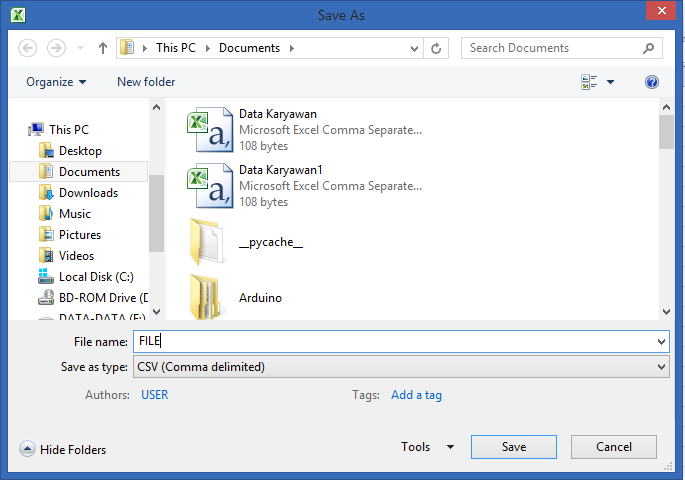
\includegraphics[width=9cm]{gambar/5.png}
    \end{center}   
    \end{figure}
      \item[f.]setelah itu  klik yes seperti pada gambar dibawah.
     \begin{figure}[!htbp]
    \begin{center}
    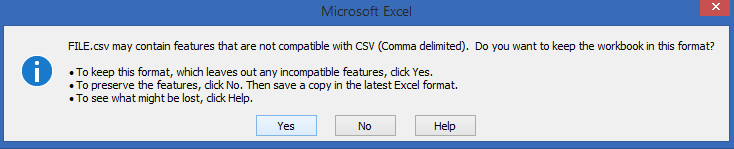
\includegraphics[width=9cm]{gambar/7.png}
    \end{center}   
    \end{figure}
    \newpage
     \item[g.].  setelah semua proses telah selesai maka file anda dengan extensi CSV sudah tersimpan, dan untuk membuka filenya  antaralain sebagai berikut:
       \begin{figure}[!htbp]
    \begin{center}
    
\includegraphics[width=5cm]{gambar/8.png}
    \end{center}   
    \end{figure}
     \begin{enumerate}
         \item [1]membuka file dengan menggunakan tekse editor(notepad), yang pertama klik kanan pada file yang telah dibuat tadi lalu pilih open with lalu pilih notepad, maka tampilannya pada notepad dapat dilihat pada ganbar dibawah.
     \begin{figure}[!htbp]
    \begin{center}
    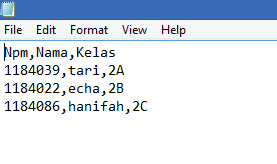
\includegraphics[width=9cm]{gambar/9.png}
    \end{center}   
    \end{figure}
    \newpage
     \item [2]membuka file dengan menggunakan Microsoft excel atau Spreadsheet, klik dua kali pada file yang dibuat , setelah itu akan  muncul tampilan seperti pada gambar dibawah.
     \begin{figure}[!htbp]
    \begin{center}
    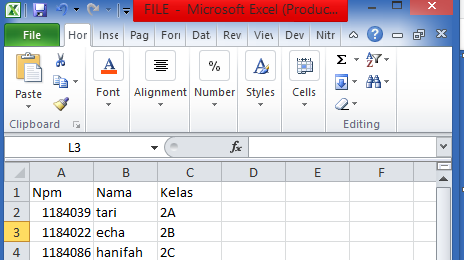
\includegraphics[width=9cm]{gambar/1.png}
    \end{center}   
    \end{figure}
     \end{enumerate}
\end{enumerate}
\section{sejarah library csv}
\hspace*{1cm}Library CSV mengimplementasikan kelas untuk membaca dan menulis data tabular dalam format CSV. Hal ini memungkinkan programmer untuk mengatakan, "tulis data ini dalam format yang disukai oleh Excel," atau "baca data dari file ini yang dihasilkan oleh Excel," tanpa mengetahui detail yang tepat dari format CSV yang digunakan oleh Excel. Pemrogram juga dapat menggambarkan format CSV yang dipahami oleh aplikasi lain atau menentukan format CSV tujuan khusus mereka sendiri.
\section{sejarah library pandas}
\hspace*{1cm}	Pandas (python Data Analysis Library) adalah distribusi atau modul opensouce  dari python untuk melakukan data manajemen dari data analisis.pandas diciptakan oleh  Wes Mckinney pada sekitaran tahun 2008, dan diperbaharui lagi oleh salah satu Koleganya yaitu Sien Chang pada tahun 2010.pandas mulai terbentuk dari  kebutuhan komunitas pengguna opensource khususnya python  yang terdapat pada package khusus yang berguna untuk melakukan  annalisis data seperti import dan export data,serta melakukan manipulasi data dan lain sebagainyaa. 
\newpage
\section{fungsi-fungsi dari library csv}
\begin{enumerate}
    \item [1]  reader.cvv adalah membaca data yang ada pada file CSV
\item[2] write.csv adalah  menulis data pada file CSV
\item[3] dictreader , adalah berfungsi untuk membaca file CSV yang ada pada dictionary
\item[4] dictwriter, adalah  berfungsi untuk menulis file csv pada  dictionary
\end{enumerate}
\section{7.fungsi yang terdapat pada pandas library}
\begin{enumerate}
    \item[1] readcsv,berfungsi untuk membaca file berformat CSV
\item[2] to csv, berfungsi untuk menulis file berformat csv
\end{enumerate}
\chapter{Keterampilan Pemrograman}
\subsection*{Soal 1}
	\lstinputlisting[firstline=10, lastline=15]{src/1184022csv.py}
\subsection*{Soal 2}
    	\lstinputlisting[firstline=17, lastline=22]{src/1184022csv.py}
\subsection*{Soal 3}
    	\lstinputlisting[ firstline=11, lastline=13]{src/1184022pandas.py}
\subsection*{Soal 4}
    	\lstinputlisting[ firstline=16, lastline=19]{src/1184022pandas.py}
\subsection*{Soal 5}
    	\lstinputlisting[ firstline=22, lastline=24]{src/1184022pandas.py}
\subsection*{Soal 6}
		\lstinputlisting[ firstline=27, lastline=30]{src/1184022pandas.py}
\subsection*{Soal 7}
    	\lstinputlisting[ firstline=33, lastline=36]{src/1184022pandas.py}
\subsection*{Soal 8}
    	\lstinputlisting[ firstline=8, lastline=11]{src/main.py}
\subsection*{Soal 9}
    \lstinputlisting[firstline=14, lastline=17]{src/main.py}

\chapter{Keterampilan Penanganan Error}
	Penanganan  errorchapter 4 ini, dapat dilihat  yaitu sebagai berikut:
\begin{enumerate}
  		\item Syntax Errors\\
		Syntax error adalah suatu keadaan atau kondisi ketika ada kesalahan penulisan kode pada program python hal ini menyebabkan program tidak dapat dijalankan. contohnya kesalahan pemberian titik dua atau tanda kutip. Output pemberitahuan error nya yaitu invalid syntax. Yang harus dilakukan saat terjadi syntax error pada kode program yaitu memperbaiki penulisan kodenya.
		
		\item Name Error\\
		NameError adalah exception yang terjadi saat kode melakukan eksekusi terhadap local name atau global name yang tidak terdefinisi. Cara mengatasi name error adalah memastikan variabel atau function yang dipanggil ada atau tidak salah ketik.
		
		\item Type Error\\
		TypeError adalah exception yang akan terjadi apabila pada saat dilakukannya eksekusi terhadap suatu operasi atau fungsi dengan type object yang tidak sesuai. cara mengatasi dari error ini adalah mengkoversi varibelnya sesuai dengan tipe data yang akan digunakan.
		
		\item Identation error\\
        Identation error, yaitu tulisasn kode program yang menjorok. identation error akan terjadi ketika mengetik kode program namun tidak memperhatikan identasinya. Jika terjadi identasi maka program akan error. cara mengatasinya yaitu memperhatikan identasi saat menuliskan suatu program.
\end{enumerate}
\newpage
	\item Penanganan Error Try except
	\lstinputlisting[firstline=1, lastline=15]{src/TryError.py}